\documentclass[12pt]{article}
\usepackage{graphicx} 
\usepackage[margin = 1in]{geometry}

\usepackage{natbib}
\usepackage{amsmath,amssymb,amsthm}
\usepackage{hyperref}
\usepackage{mathtools}
\newcommand{\ind}{\perp\!\!\!\!\perp} 
\DeclareMathOperator{\D}{D}
\DeclareMathOperator{\E}{\mathbb{E}}
\DeclareMathOperator{\Var}{Var}
\theoremstyle{definition}
\newtheorem{assumption}{Assumption}
\usepackage{setspace}
\doublespacing

\title{Using Normalizing Flows for Weighting Estimators with Continuous Treatment}
\author{Chanhyuk Park \qquad Xiangyu Song}
\date{\today}

\begin{document}

\maketitle

\begin{abstract}
  
\end{abstract}

\clearpage


\section{Introduction}

In observational studies, political scientists care about an unbiased estimator for average treatment effect (ATE) or average treatment effect on the treated (ATT). One way to generate an unbiased and also semiparametrically efficient estimator is by using augmented inverse propensity weighting(AIPW) estimator, known to be doubly robust. However, there are two caveats here. First, as continuous treatment is common in political science studies, simply dichotomizing treatments to fit into AIPW with a binary treatment framework may lose information on the treatment effect heterogeneity. Second, although researchers can use logit or probit to estimate the propensity score with binary treatment easily, an accurate estimation of the propensity score under continuous treatment is still a challenge. In this paper, we propose to use the normalizing flows (NF), which produce efficient and exact propensity score estimation with continuous treatment.


\section{Related Literature}


\subsection{Continuous Treatment and Generalized Propensity Score}

A large literature studies the inference for various treatment effects with binary or categorical treatments, either with randomized experiment or observational studies. In political science, such examples include the Get Out the Vote (GOTV) campaign on voter turnout \citep{gerber2000effects}, the effect of product differentiation in economic markets on firm-level lobbying in political markets \citep{kim2017political}, and the effect of patron-client network on economic development in China \citep{jiang2018making}. However, many empirical settings could also involve continuous treatment, such as the campaign spending, the intensity of a policy implementation, as well as the media exposure. In such settings, causal effects are naturally summarized by an average dose-response function, or the average structural function \citep{colangelo2026double}.
\begin{align*}
  m(t) = \E \left[  Y(t) \right], 
\end{align*}
rather than by a single average treatment effect. Under consistency, overlap, and conditional ignorability assumption, this curve can be identified as 
\begin{align*}
  m(t) = \E \left[ \mu(X, t) \right], \qquad \mu(x, d) = \E \left[ Y \mid X = x, T = t \right].
\end{align*}
\citet{hirano2004propensity} provide the foundational propensity-score approach for continuous treatment: the generalized propensity score (GPS). Defined as 
\begin{align*}
  g(t \mid x) = f_{T \mid X} (t \mid x),
\end{align*}
GPS is the conditional density of the treatment given the covariates. They have shown that the GPS plays an analogous balancing role to the binary propensity score. Although their framework provides a way to estimate does-response functions by adjusting for the GPS, it often relies on parametric modeling of the treatment density.


\subsection{Semiparametric Theory and Doubly Robust Estimators}

As mentioned by \citet{kennedy2017nonparametric}, semiparametric theory is not directly available if we only assume mild smoothness conditions on $\theta(d)$ (e.g., differentiability) since without parametric assumptions $\theta(d)$ is not pathwise differentiable, and root $n$ consistent estimators do not exist. By defining a parameter that represents the average outcome under an intervention that randomly assigns treatment based on the density of the continuous treatment, \citet{kennedy2017nonparametric} construct the efficient influence function for this stochastic-intervention parameter, which contains a pseudo-outcome term that attains the double robustness.

\section{Problem Setup}


%\section{Augmented Inverse Propensity Weighting}

%In observational studies, the key assumption is the unconfoundedness. Formally, let $X_i$ denote a vector of pretreatment variables or covariates, $D_i$ denote the treatment, and $Y_{i}(0), Y_{i}(1)$ denote the potential outcomes. We assume that the treatment is independent of the potential outcomes given $X_i$.
%\begin{assumption}[Unconfoundedness]\label{asm1}
%    \[ D_i \ind \left(Y_{i}(0), Y_{i}(1) \right) \mid X_i\]
%\end{assumption}
%In applications, when the dimension of pretreatment variables $X_i$ is substantial, conditioning on $X_i$ can be a challenge. One key result from \citet{rosenbaum1983central} shows that Assumption \ref{asm1} implies
%\[ D_i \ind \left(Y_{i}(0), Y_{i}(1) \right) \mid e(X_i), \]
%where $e(\cdot)$ is the propensity score that plays a key role in observational studies.
%
%To identify the average causal effect under unconfoundedness, we also need to ensure that we can estimate the average effect at every value of the covariates, requiring overlap, that guarantees that the treatment assignment probability is bounded away from zero and one.
%\begin{assumption}[Overlap]\label{asm2}
%    \[0 < e(X_i) \equiv \Pr(D_i = d \mid X_i = x) < 1.\]
%\end{assumption}
% %\citet{rosenbaum1983central} refer these two assumptions as the strong ignorability.  
%To estimate the causal effect of interest, e.g., ATE or ATT, a variety of methods have been proposed under the unconfoundedness and overlap assumptions, referred as strong ignorability by \citet{rosenbaum1983central}. \citet{imbens2024lalonde} summarise these methods into three groups. In addition to outcome modeling and inverse propensity weighting (IPW), we focus on the AIPW estimator that improves the small sample performance by combining outcome modeling with methods addressing covariate imbalance to eliminate remaining biases or improve precision.

%The first one is outcome modeling. Define the conditional expectation of the two potential outcomes given treatment and covariates as
%\[ \mu_d(x) = \mathbb{E}[Y_i(d) \mid X_i = x], \quad \text{where} \quad d \in \{0, 1\}.  \]
%Then, under the unconfoundedness assumption, we can define the population ATE as 
%\[\tau^{\text{pop}} = \mathbb{E}[\mu_1(X) - \mu_0(X)].\]
%
%The second group of methods focuses on adjusting covariate imbalance between the treatment and control groups. Among various blocking, matching, and reweighting methods, inverse propensity weighting (IPW) leverages the propensity score instead of simple covariate matching, which suffers from the curse of dimensionality. Rather than viewing the propensity score as a balancing score, exploiting the interpretation as the probability of being exposed to the treatment gives the following result when assuming unconfoundedness:
%\[ \mathbb{E}\left[ \frac{DY}{e(X)} \right] = \mathbb{E}[Y(1)], \quad \mathbb{E}\left[ \frac{(1 - D)Y}{1 - e(X)} \right] = \mathbb{E}[Y(0)]  .\]
%Reweighting the units by the inverse of propensity score, we can get the sample analogy of the ATE:
%\[ \hat{\tau}_{\text{IPW}} = \frac{1}{n} \sum_{i = 1}^{n} \left[ \frac{D_iY_i}{\hat{e}(X_i)} - \frac{(1 - D_i)Y_i}{1 - \hat{e}(X_i)} \right], \]
%where $\hat{e}(X_i)$ is the estimated propensity score. When the propensity is known, then this IPW estimator is unbiased for the ATE, and if propensity scores are estimated consistently, then this estimator is consistent for ATE. However, such a simple IPW estimator is believed to have poor small sample properties when the propensity score gets close to zero or one for some observations \citep{glynn2010introduction}. 

%\citet{abadie2011biascorrecteda} provide the example that while the bias of a simple matching estimator might dominate variance in high-dimensional cases, adding regression to account for the remaining imbalance can substantially reduce such biases. The AIPW estimator for ATE with a binary treatment $D$ is as the following:
%\begin{equation}\label{AIPW}
%    \begin{aligned}
%    \tau_{\text{AIPW}} &= \mu_1(X) - \mu_0(X) + \frac{(Y - \mu_1(X)) D}{e(X)} - \frac{(Y - \mu_0(X) (1 - D)}{1 - e(X)}\\
%    &= \frac{DY}{e(X)} - \frac{(1 - D) Y}{1 - e(X)} + \frac{e(X) - D}{e(x) (1 - e(x))} \left[\mu_1(X)(1 - e(X)) + \mu_0(X)e(X)\right].
%    \end{aligned}
%\end{equation}
%We can get the sample analogy as 
%\begin{align*}
%    \hat{\tau}_{\text{AIPW}} = \frac{1}{n} \sum_{i = 1}^{n} \left\{ \frac{D_iY_i}{\hat{e}(X_i)} - \frac{(1 - D_i) Y_i}{1 - \hat{e}(X_i)} + \frac{\hat{e}(X_i) - D_i}{\hat{e}(X_i) (1 - \hat{e}(X_i))} \left[\mu_1(X_i)(1 - \hat{e}(X_i)) + \mu_0(X_i)\hat{e}(X_i)\right] \right\}.
%\end{align*}
%The AIPW estimators can be viewed as combining an outcome model with an adjustment term, which consists of an IPW estimator applied to the residuals from the outcome model, as shown in Equation \ref{AIPW}. \citet{robins1997curse} use the term ``double robustness'' for these mixed methods. If either the propensity score or regression model is correctly specified parametrically, the AIPW estimator that combines weighting and regression is consistent.
%
%To get the unbiased AIPW estimator, researchers need to estimate the propensity score. When the treatment is binary, fitting a logit or probit model can provide the estimated propensity score. However, when the treatment is multinomial or continuous, we need more tools for the estimation. Here our focus is the continuous treatment, which is quite common in the political science setting. Existing studies mostly use kernel density estimation (KDE) technique for the estimation of propensity score. However, KDE largely depends on the chosen kernel and bandwidth. In the paper, we are proposing to use the NF, which are generative models that produce tractable distributions where both sampling and density evaluation can be efficient and exact for propensity score estimation \citep{kobyzev2021normalizing}. 


\section{Normalizing Flows}
NF are generative models which produce tractable distributions where both sampling and density evaluation can be efficient and exact, using invertible functions. In other words, it is a technique that maps a random variable with a complex probability density function to the simpler density function.

A typical NF procedure starts with a simple base distribution such as Gaussian and then attempts to transform that function into a more complex distribution by applying a finite number of invertible functions\footnote{The existence of this process is always guaranteed, and discussed in \citet{Chen2000a}.}. The process utilized the \textit{change of variables formula}, which guarantees mapping of one probability density function for a random variable $Y$ with another probability density function of random variable $Z$:
$$
\begin{aligned}
    p_{\mathbf{Y}}(\mathbf{y}) &= p_{\mathbf{Z}}(\mathbf{f}(\mathbf{y}))| \det \D\mathbf{f}(\mathbf{y}) | \\
           &= p_{\mathbf{Z}}(\mathbf{f}(\mathbf{y}))| \det \D\mathbf{g}(\mathbf{f}(\mathbf{y})) |^{-1},
\end{aligned}
$$
where $\mathbf{g}$ is an invertible function, $\mathbf{f} = \mathbf{g}^{-1}$, and $\D\mathbf{f}(\mathbf{y}) = \frac{\partial \mathbf{f}}{\partial \mathbf{y}}$ is the Jacobian of $\mathbf{f}$. Figure \ref{fig:nf_graph} illustrates this relationship. Since $\mathbf{f}$ moves in the direction of a simple base distribution, it is called \textit{normalizing flow}. 

\begin{figure}[h]
    \centering
    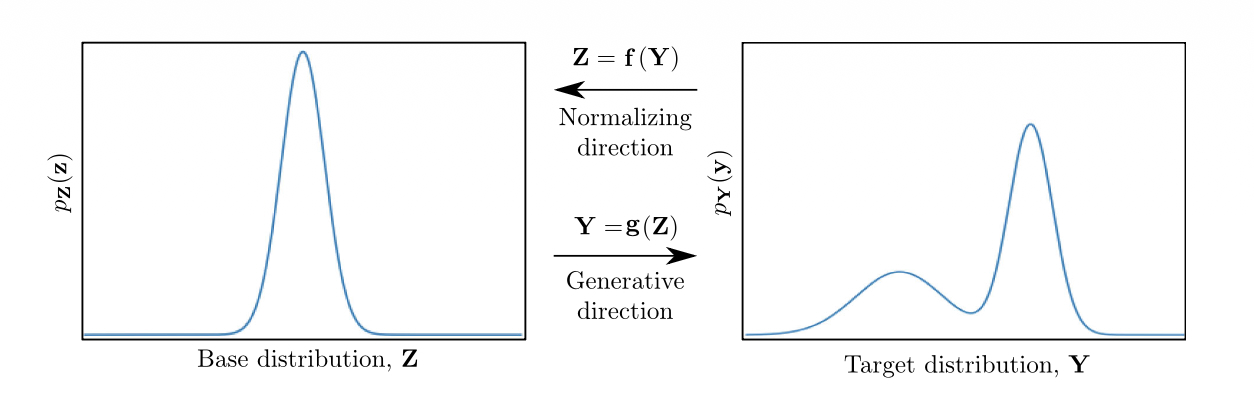
\includegraphics[width=0.8\linewidth]{../figures/nf_graph.jpg}
    \caption{Graphical Illustration of Normalizing Flows. from \cite{kobyzev2021normalizing}}
    \label{fig:nf_graph}
\end{figure}

As a result of this process, we can link the complex distribution (such as a joint distribution of variables we observe) with simple base distribution such as Gaussian. Since this is an invertible process, instead of dealing with the complex distribution itself, we can work with the simple base distribution such as sampling and density estimation, and then easily bring the result to the complex one.

NF is a useful tool in density estimation compare to other frequently used density estimation method. Histogram is  a simple exploratory method. However, it relies heavily on the size of bins and thus often performs poorly on complex distributions. Unlike the histogram, KDE technique produces a smooth estimate of the density, using all sample points' locations. The main idea behind KDE has been proposed long ago \citep{Rosenblatt1956a}, but the recent development of computing technology makes it a popular option today. KDE, however, requires researchers to decide which kernel to be used and the size of the bandwidth, and both influence the estimation result. Since NF usually relies on neural network, the computational cost may be high for complex design, it is more capable of dealing with complex density.

\section{Using NF for Propensity Score Estimation}
One straight forward application of density estimation with NF is propensity score estimation. Statistical estimators employing propensity score relies heavily on the accuracy of the propensity score. 

Although there are criticism on using machine learning algorithm in propensity score estimation, it becomes more popular \citep{Goller2020a}. \citet{Lechner2024a} utillized random forest estimation of propensity score. In this paper, we propose to use NF as an alternative for propensity score estimation and leverage the estimated propensity score into the AIPW estimator in observational studies.



\clearpage
\bibliography{ref}
\bibliographystyle{ecta}

\end{document}
